\documentclass{article}
\usepackage{amsmath}
\usepackage{graphicx}
\begin{document}
\title{Coordinate Geometry Unit Exam: Question 48}
\author{Ana Bhattacharjee}
\date{\today}
\maketitle{}

\begin{center}
To use the slopes of the sides of the figure below, we must do the following to prove it is a right triangle:
\begin{itemize}
  \item Compute both slopes
  \item Ensure their product is equivalent to -1
\end{itemize}
By seeing their product is negative 1, we can prove the two slopes are perpendicular hence creating a 90$^\circ$ angle.
\begin{figure}[!htbp]
  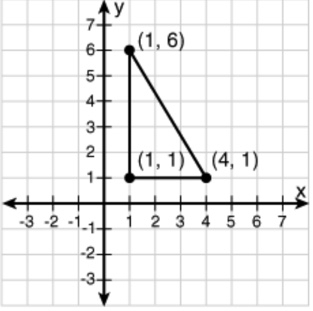
\includegraphics[width=1.0\columnwidth]{triangle}
  \caption{Triangle in Coordinate Plane}
\end{figure}
\par
The slope of the vertical leg is :
\begin{align}
  \frac{6 - 1}{1 - 1} \rightarrow \text{undefined}
\end{align}
The slope of the horizontal leg is :
\begin{align}
  \frac{1 - 1}{4 - 1} = 0
\end{align}
An undefined slope and a slope equal to 0 are perpendicular just as an x axis and a y axis are perpendicular to each other. Therefore, the triangle is a right triangle. 
\end{center}
\end{document}
